\input preamble.tex

% set up externalization
%\usetikzlibrary{external}
%\tikzset{external/system call={latex \tikzexternalcheckshellescape -halt-on-error
%-interaction=batchmode -jobname "\image" "\texsource";
%dvips -o "\image".ps "\image".dvi;
%ps2eps "\image.ps"}}
%\tikzexternalize

\begin{document}
\begin{tikzpicture}[scale=0.6]
\coordinate (I0) at (0,0);
\coordinate (I1) at (3,5);
\coordinate (I2) at (-11,-2.5);
% right ground 2
    \shade[shaderect] ([shift={(-3,-1)}]I2) rectangle ([shift={(+3,+1)}]I2);
    \draw[rect]  ([shift={(-3,-1)}]I2) rectangle ([shift={(+3,+1)}]I2);
    \node (ground2) at ([shift={(0,-1)}]I2) [ground2,anchor=north] {};
    \draw[rect] (ground2.north west) -- (ground2.north east);
% left ground 1
    \shade[shaderect] ([shift={(0.32,0)}]I0) rectangle ([shift={(-0.32,-1)}]I0);
    \draw[rect] ([shift={(0.32,0)}]I0) rectangle ([shift={(-0.32,-1)}]I0);
    \node (ground1) at ([shift={(0,-1)}]I0) [ground1,anchor=north] {};
    \draw[rect] (ground1.north west) -- (ground1.north east);
% right arm
    \draw[arm] (I1) -- (I2);
% left arm
    \draw[arm] (I0) -- (I1);
% vector
    \draw[vec] (I1) -- (I2) node[midway,above left,yshift=3pt] {$\bar{r}_3$};
    \draw[vec] (I0) -- (I1) node[midway,below right,yshift=-3pt,xshift=2pt] {$\bar{r}_2$};
    \draw[vec] (I0 |- I2) -- (I2) node[below,midway] {$\bar{r}_4$};
    \draw[vec] (I0) -- (I0 |- I2) node[near end,right] {$\bar{r}_1$};
% xy axis
    \draw[axis] (I0) -- ([shift={(5,0)}]I0) node[below] {$x$};
    \draw[axis] (I0) -- ([shift={(0,5)}]I0) node[left] {$y$};
% angle
    \draw[vecax] let \p1 = (I1) in (I1) -- +(0:1.5);
    \draw[vec] let \p1 = (I1), \p2 = (I2) in ([shift={(1,0)}]I1) arc (0:270+(atan((\x2-\x1)/(\y1-\y2))):1) node[midway,above] {$\theta_3$};
    \draw[vec] let \p1 = (I1) in ([shift={(1,0)}]I0) arc (0:(atan(\y1/\x1):1) node[midway,right] {$\theta_2$};
\end{tikzpicture}
\end{document}
\centering
\pagestyle{empty}
\newcommand{\imagetik}[1]{\null\vfill\includegraphics[width=0.8\textwidth]{draw#1.pdf}\vfill\null\clearpage}
\imagetik{1}
\imagetik{2}
\imagetik{3}
\imagetik{4}
\imagetik{5}
\imagetik{6}
\imagetik{7}
\imagetik{8}
\imagetik{9}

\end{document}

\includegraphics{tikzpicture-figure0.eps}
\includegraphics{tikzpicture-figure1.eps}
\includegraphics{tikzpicture-figure2.eps}
\includegraphics{tikzpicture-figure3.eps}
\includegraphics{tikzpicture-figure4.eps}
\includegraphics{tikzpicture-figure5.eps}
\includegraphics{tikzpicture-figure6.eps}
\includegraphics{tikzpicture-figure7.eps}
\includegraphics{tikzpicture-figure8.eps}

\end{document}
% Draw:1
% Schematic of offset slider-crank
\begin{figure}[!ht]
\centering
\footnotesize
\begin{tikzpicture}[scale=0.6]
\coordinate (I0) at (0,0);
\coordinate (I1) at (3,5);
\coordinate (I2) at (17,-2.5);
% right ground 2
    \shade[shaderect] ([shift={(-3,-1)}]I2) rectangle ([shift={(+3,+1)}]I2);
    \draw[rect]  ([shift={(-3,-1)}]I2) rectangle ([shift={(+3,+1)}]I2);
    \node (ground2) at ([shift={(0,-1)}]I2) [ground2,anchor=north] {};
    \draw[rect] (ground2.north west) -- (ground2.north east);
% left ground 1
    \shade[shaderect] ([shift={(0.32,0)}]I0) rectangle ([shift={(-0.32,-1)}]I0);
    \draw[rect] ([shift={(0.32,0)}]I0) rectangle ([shift={(-0.32,-1)}]I0);
    \node (ground1) at ([shift={(0,-1)}]I0) [ground1,anchor=north] {};
    \draw[rect] (ground1.north west) -- (ground1.north east);
% right arm
    \draw[arm] (I1) -- (I2);
% left arm
    \draw[arm] (I0) -- (I1);
% vector
    \draw[vec] (I1) -- (I2) node[midway,above right,yshift=3pt] {$\bar{r}_3$};
    \draw[vec] (I0) -- (I1) node[midway,above left,yshift=3pt,xshift=-2pt] {$\bar{r}_2$};
    \draw[vec] (I0 |- I2) -- (I2) node[below,midway] {$\bar{r}_4$};
    \draw[vec] (I0) -- (I0 |- I2) node[near end,left] {$\bar{r}_1$};
% xy axis
    \draw[axis] (I0) -- ([shift={(5,0)}]I0) node[below] {$x$};
    \draw[axis] (I0) -- ([shift={(0,5)}]I0) node[left] {$y$};
% angle
    \draw[vecax] let \p1 = (I1) in (I1) -- +(0:1.5);
    \draw[vec] let \p1 = (I1), \p2 = (I2) in ([shift={(1,0)}]I1) arc (0:270+(atan((\x2-\x1)/(\y1-\y2))):1) node[midway,left] {$\theta_3$};
    \draw[vec] let \p1 = (I1) in ([shift={(1,0)}]I0) arc (0:(atan(\y1/\x1):1) node[midway,right] {$\theta_2$};
\end{tikzpicture}
\caption{Schematic of offset slider-crank}\label{Draw:1}
\end{figure}

\clearpage
% Draw:2
% Schematic of second possible solution for position equation
\begin{figure}[!ht]
\centering
\footnotesize
\begin{tikzpicture}[scale=0.6]
\coordinate (I0) at (0,0);
\coordinate (I1) at (3,5);
\coordinate (I2) at (-11,-2.5);
% right ground 2
    \shade[shaderect] ([shift={(-3,-1)}]I2) rectangle ([shift={(+3,+1)}]I2);
    \draw[rect]  ([shift={(-3,-1)}]I2) rectangle ([shift={(+3,+1)}]I2);
    \node (ground2) at ([shift={(0,-1)}]I2) [ground2,anchor=north] {};
    \draw[rect] (ground2.north west) -- (ground2.north east);
% left ground 1
    \shade[shaderect] ([shift={(0.32,0)}]I0) rectangle ([shift={(-0.32,-1)}]I0);
    \draw[rect] ([shift={(0.32,0)}]I0) rectangle ([shift={(-0.32,-1)}]I0);
    \node (ground1) at ([shift={(0,-1)}]I0) [ground1,anchor=north] {};
    \draw[rect] (ground1.north west) -- (ground1.north east);
% right arm
    \draw[arm] (I1) -- (I2);
% left arm
    \draw[arm] (I0) -- (I1);
% vector
    \draw[vec] (I1) -- (I2) node[midway,above left,yshift=3pt] {$\bar{r}_3$};
    \draw[vec] (I0) -- (I1) node[midway,below right,yshift=-3pt,xshift=2pt] {$\bar{r}_2$};
    \draw[vec] (I0 |- I2) -- (I2) node[below,midway] {$\bar{r}_4$};
    \draw[vec] (I0) -- (I0 |- I2) node[near end,right] {$\bar{r}_1$};
% xy axis
    \draw[axis] (I0) -- ([shift={(5,0)}]I0) node[below] {$x$};
    \draw[axis] (I0) -- ([shift={(0,5)}]I0) node[left] {$y$};
% angle
    \draw[vecax] let \p1 = (I1) in (I1) -- +(0:1.5);
    \draw[vec] let \p1 = (I1), \p2 = (I2) in ([shift={(1,0)}]I1) arc (0:270+(atan((\x2-\x1)/(\y1-\y2))):1) node[midway,above] {$\theta_3$};
    \draw[vec] let \p1 = (I1) in ([shift={(1,0)}]I0) arc (0:(atan(\y1/\x1):1) node[midway,right] {$\theta_2$};
\end{tikzpicture}
\caption{Schematic of second possible solution for position equation}\label{Draw:2}
\end{figure}

\clearpage
% Draw:3
% Schematic of system for energy analysis
\begin{figure}[!ht]
\centering
\footnotesize
\begin{tikzpicture}[scale=0.6]
\coordinate (I0) at (0,0);
\coordinate (I1) at (3,5);
\coordinate (I2) at (17,-2.5);
% right ground 2
    \shade[shaderect] ([shift={(-3,-1)}]I2) rectangle ([shift={(+3,+1)}]I2);
    \draw[rect]  ([shift={(-3,-1)}]I2) rectangle ([shift={(+3,+1)}]I2);
    \node (ground2) at ([shift={(0,-1)}]I2) [ground2,anchor=north] {};
    \draw[rect] (ground2.north west) -- (ground2.north east);
% left ground 1
    \shade[shaderect] ([shift={(0.32,0)}]I0) rectangle ([shift={(-0.32,-1)}]I0);
    \draw[rect] ([shift={(0.32,0)}]I0) rectangle ([shift={(-0.32,-1)}]I0);
    \node (ground1) at ([shift={(0,-1)}]I0) [ground1,anchor=north] {};
    \draw[rect] (ground1.north west) -- (ground1.north east);
% right arm
    \draw[arm] (I1) -- (I2);
% left arm
    \draw[arm] (I0) -- (I1);
% vector
    \draw[vec] (I1) -- (I2) node[midway,above right,yshift=3pt] {$\bar{r}_3$};
    \draw[vec] (I0) -- (I1) node[midway,above left,yshift=3pt,xshift=-2pt] {$\bar{r}_2$};
    \draw[vec] (I0 |- I2) -- (I2) node[below,midway] {$\bar{r}_4$};
    \draw[vec] (I0) -- (I0 |- I2) node[near end,left] {$\bar{r}_1$};
% xy axis
    \draw[axis] (I0) -- ([shift={(5,0)}]I0) node[below] {$x$};
    \draw[axis] (I0) -- ([shift={(0,5)}]I0) node[left] {$y$};
% angle
    \draw[vecax] let \p1 = (I1) in (I1) -- +(0:1.5);
    \draw[vec] let \p1 = (I1), \p2 = (I2) in ([shift={(1,0)}]I1) arc (0:270+(atan((\x2-\x1)/(\y1-\y2))):1) node[midway,left] {$\theta_3$};
    \draw[vec] let \p1 = (I1) in ([shift={(1,0)}]I0) arc (0:(atan(\y1/\x1):1) node[midway,right] {$\theta_2$};
% cross circle 2 /2
\coordinate (c2) at ($(I0)!0.5!(I1)$);
\sysan{c2}
% cross circle 3 /2 
\coordinate (c3) at ($(I1)!0.5!(I2)$);
\sysan{c3}
% cross circle 3 end
\sysan{I2}
\end{tikzpicture}
\caption{Schematic of system for energy analysis}\label{Draw:3}
\end{figure}

% Draw:4
% Schematics of six-bar linkage to represent cyclist and crank system
\begin{figure}[!ht]
\centering
\footnotesize
\begin{tikzpicture}[scale=0.5]
\coordinate (I0) at (0,-2);
\coordinate (I1) at (0,20);
\coordinate (I2) at (7,16);
\coordinate (I3) at (3,6);
\coordinate (I4) at (8,3);
\coordinate (I5) at (5,-2);
\coordinate (VS) at (30,0);
% arms
    \draw[arm] (I0) -- (I1) node [midway,left,xshift=-5pt] {$I_6$};
    \draw[arm] (I1) -- (I2) node [midway,above,yshift=6pt] {$I_1$};
    \draw[arm] (I2) -- (I3) node [midway,right,xshift=5pt] {$I_2$};
    \draw[arm] (I3) -- (I4) node [midway,above,yshift=6pt] {$I_3$};
    \draw[arm] (I4) -- (I5) node [midway,right,xshift=5pt] {$I_4$};
    \draw[arm] (I5) -- (I0) node [midway,below,yshift=-5pt] {$I_5$};
% arc 1
    \draw[vecax] let \p1 = (I1), \p2 = (I2) in (I1) -- +({-atan((\y1-\y2)/(\x2-\x1))}:1.5);
    \draw[vec] let \p1 = (I1), \p2 = (I2) in ([shift={(0,-1)}]I1) arc (-90:-atan((\y1-\y2)/(\x2-\x1)):1) node[midway,below right,xshift=-2pt] {$\theta_1$};
% arc 2
    \draw[vecax] (I2) -- +(-90:1.5);
    \draw[vecax] let \p2 = (I2), \p3 = (I3) in (I2) -- +({270-atan((\x2-\x3)/(\y2-\y3))}:1.5);
    \draw[vec] let \p2 = (I2), \p3 = (I3) in ([shift={(0,-1)}]I2) arc (-90:270-atan((\x2-\x3)/(\y2-\y3)):1) node[midway,above] {$\theta_2$};
% arc 3
    \draw[vecax] (I3) -- +(-90:1.5);
    \draw[vecax] let \p3 = (I3), \p4 = (I4) in (I3) -- +({-atan((\y3-\y4)/(\x4-\x3))}:1.5);
    \draw[vec] let \p3 = (I3), \p4 = (I4) in ([shift={(0,-1)}]I3) arc (-90:-atan((\y3-\y4)/(\x4-\x3)):1) node[midway,below,xshift=2pt] {$\theta_3$};
% arc 4
    \draw[vecax] (I5) -- +(-90:1.5);
    \draw[vecax] let \p4 = (I4), \p5 = (I5) in (I5) -- +({atan((\y4-\y5)/(\x4-\x5))}:1.5);
    \draw[vec] let \p4 = (I4), \p5 = (I5) in ([shift={(0,-1)}]I5) arc (-90:atan((\y4-\y5)/(\x4-\x5)):1) node[midway,right] {$\theta_4$};
% arc 5
    \draw[vecax] (I0) -- ([shift={(0,1.5)}]I0);
    \draw[vecax] (I0) -- ([shift={(1.5,0)}]I0);
    \draw[vecret] ([shift={(1,0)}]I0) -- ([shift={(1,1)}]I0) -- ([shift={(0,1)}]I0);
% vectors
    \draw[->] ([shift={(VS)}]I0) -- ([shift={(VS)}]I1) node [midway,left] {$\bar{r}_6$};
    \draw[->] ([shift={(VS)}]I1) -- ([shift={(VS)}]I2) node [midway,above] {$\bar{r}_1$};
    \draw[->] ([shift={(VS)}]I2) -- ([shift={(VS)}]I3) node [midway,right] {$\bar{r}_2$};
    \draw[->] ([shift={(VS)}]I3) -- ([shift={(VS)}]I4) node [midway,above] {$\bar{r}_3$};
    \draw[->] ([shift={(VS)}]I4) -- ([shift={(VS)}]I5) node [midway,right] {$\bar{r}_4$};
    \draw[->] ([shift={(VS)}]I5) -- ([shift={(VS)}]I0) node [midway,below] {$\bar{r}_5$};
% xy axis
    \draw[axis] (I1) -- ([shift={(0,-5)}]I1) node[left,xshift=-5pt] {$x$};
    \draw[axis] (I1) -- ([shift={(5,0)}]I1) node[above,yshift=3pt] {$y$};
\end{tikzpicture}
\caption{Schematics of six-bar linkage to represent cyclist and crank system}\label{Draw:4}
\end{figure}

\clearpage
% Draw:5
% Schematic of pedal and crank angle relations
\begin{figure}[!ht]
\centering
\footnotesize
\begin{tikzpicture}[scale=0.5]
\clip (0.9,-3.5) rectangle (9.05,9);
\coordinate (I0) at (0,-2);
\coordinate (I1) at (0,20);
\coordinate (I2) at (7,16);
\coordinate (I3) at (3,6);
\coordinate (I4) at (8,3);
\coordinate (I5) at (5,-2);
\coordinate (VS) at (30,0);
% arms
    \draw[arm,gray] (I2) -- (I3) node [near end,right,xshift=5pt] {$I_2$};
    \draw[arm,gray] (I5) -- (I0) node [midway,below,yshift=-5pt] {$I_5$};
    \draw[arm] (I3) -- (I4) node [midway,above,yshift=7pt] {$I_3$};
    \draw[arm] (I4) -- (I5) node [midway,right,xshift=6pt] {$I_4$};
% arc
    \centerarc[gray,dashdotted](I5)(0:180:sqrt(34))
% triangle
    \draw[triangle] (I3) -- (I4) -- (I3 |- I4) -- (I3);
% arc 3
    \draw[vec] let \p3 = (I3), \p4 = (I4) in ([shift={(0,-1)}]I3) arc (-90:-atan((\y3-\y4)/(\x4-\x3)):1) node[midway,below,xshift=1pt] {$\theta_3$};
% arc pedal
    \draw[->] ([shift={(-1,0)}]I4) arc (180:180-atan(3/5):1) node[midway,left,xshift=-7pt,yshift=1pt] {$\theta_\text{pedal}$};
% arc 4
    \draw[vecax] (I5) -- +(-90:1.5);
    \draw[vecax] let \p4 = (I4), \p5 = (I5) in (I5) -- +({atan((\y4-\y5)/(\x4-\x5))}:1.5);
    \draw[vec] let \p4 = (I4), \p5 = (I5) in ([shift={(0,-1)}]I5) arc (-90:atan((\y4-\y5)/(\x4-\x5)):1) node[midway,right] {$\theta_\text{crank}$};
% rect angle
    \draw[vecret] (3,4) -- (4,4) -- (4,3);
\end{tikzpicture}
\caption{Schematic of pedal and crank angle relations}\label{Draw:5}
\end{figure}

\clearpage
% Draw:6
% Triangle created by the shank, projection from
\begin{figure}[!ht]
\centering
\footnotesize
\begin{tikzpicture}[scale=0.5]
\clip (0.4,3.35) rectangle (17,18.5);
\coordinate (I0) at (0,-2);
\coordinate (I1) at (0,20);
\coordinate (I2) at (7,16);
\coordinate (I3) at (3,6);
\coordinate (I4) at (8,3);
\coordinate (I5) at (5,-2);
\coordinate (VS) at (30,0);
% arms
    \draw[arm,gray] (I1) -- (I2) node [near end,above,yshift=7pt] {$I_1$};
    \draw[arm,gray] (I3) -- (I4) node [midway,below,yshift=-3pt,xshift=-3pt] {$I_3$};
    \draw[arm] (I2) -- (I3) node [midway,left,xshift=-7pt] {$I_2$};
% triangle
    \draw[triangle] (I2) -- (I3) -- (I2 |- I3) -- (I2);
% arc 2
%    \draw[vecax] (I2) -- +(-90:1.5);
%    \draw[vecax] let \p2 = (I2), \p3 = (I3) in (I2) -- +({270-atan((\x2-\x3)/(\y2-\y3))}:1.5);
    \draw[vec] let \p2 = (I2), \p3 = (I3) in ([shift={(0,-1)}]I2) arc (-90:270-atan((\x2-\x3)/(\y2-\y3)):1) node[midway,above] {$\theta_2$};
% label 
\coordinate (I23) at ($(I2)!0.5!(I3)$);
\node[below,yshift=-8pt,fill=white,inner sep=1pt] at (I23 |- I3)  {$\left({l}_{5}+{l}_{4}\sin{\theta}_{4}-{l}_{3}\sin\theta_{3}\right)-{l}_{1}\sin{\theta}_{1}$};
\node[right,xshift=6pt] at (I2 |- I23) {$\left({l}_{6}+{l}_{4}\cos\theta_{4}-{l}_{3}\cos{\theta}_{3}\right)-{l}_{1}\cos\theta_{1}$};
\end{tikzpicture}
\caption{Triangle created by the shank, projection from}\label{Draw:6}
\end{figure}

\clearpage
% Draw:7
% Schematic example of crossover in genetic algorithms
\begin{figure}[!ht]
\centering
\footnotesize
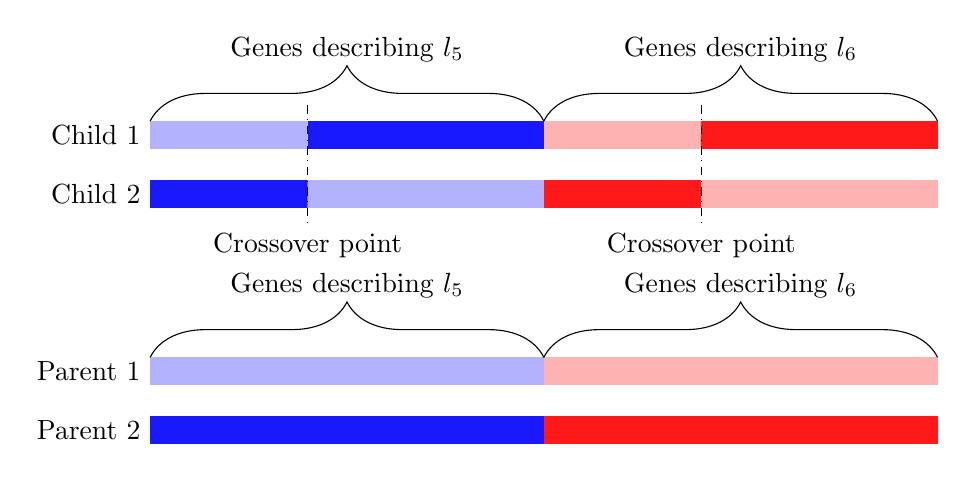
\begin{tikzpicture}[xscale=1,yscale=0.75]
\definecolor{P11}{rgb}{0.7,0.7,1}
\definecolor{P12}{rgb}{1,0.7,0.7}
\definecolor{P21}{rgb}{0.1,0.1,1}
\definecolor{P22}{rgb}{1,0.1,0.1}

\node (CPt) at (0,5.5) {};
\node (CPb) at (0,3.5) {};
\node[left] (C1) at (0,5) {Child 1};
\node[left] (C2) at (0,4) {Child 2};
\node[left] (P1) at (0,1) {Parent 1};
\node[left] (P2) at (0,0) {Parent 2};
\node (N1) at (2,0) {};
\node (N2) at (5,0) {};
\node (N3) at (7,0) {};
\node (N4) at (10,0) {};

\draw[P21,line width=10pt] (P2) -- (N2 |- P2);
\draw[P22,line width=10pt] (N2|- P2) -- (N4|- P2);

\draw[P11,line width=10pt] (P1) -- (N2 |- P1);
\draw[P12,line width=10pt] (N2 |- P1) -- (N4 |- P1);

\draw[P11,line width=10pt] (C1) -- (N1 |- C1);
\draw[P21,line width=10pt] (N1|- C1) -- (N2|- C1);
\draw[P12,line width=10pt] (N2|- C1) -- (N3|- C1);
\draw[P22,line width=10pt] (N3|- C1) -- (N4|- C1);

\draw[P21,line width=10pt] (C2) -- (N1 |- C2);
\draw[P11,line width=10pt] (N1|- C2) -- (N2|- C2);
\draw[P22,line width=10pt] (N2|- C2) -- (N3|- C2);
\draw[P12,line width=10pt] (N3|- C2) -- (N4|- C2);

\draw[dashdotted] (N1 |- CPt) -- (N1 |- CPb) node[below] {Crossover point};
\draw[dashdotted] (N3 |- CPt) -- (N3 |- CPb) node[below] {Crossover point};

\draw [decorate,decoration={brace,amplitude=20pt,raise=5pt}] (C1) -- (N2 |- C1) node [midway,above,yshift=23pt] {Genes describing $l_5$};
\draw [decorate,decoration={brace,amplitude=20pt,raise=5pt}] (N2 |- C1) -- (N4 |- C1) node [midway,above,yshift=23pt] {Genes describing $l_6$};

\draw [decorate,decoration={brace,amplitude=20pt,raise=5pt}] (P1) -- (N2 |- P1) node [midway,above,yshift=23pt] {Genes describing $l_5$};
\draw [decorate,decoration={brace,amplitude=20pt,raise=5pt}] (N2 |- P1) -- (N4 |- P1) node [midway,above,yshift=23pt] {Genes describing $l_6$};

\end{tikzpicture}
\caption{Schematic example of crossover in genetic algorithms}\label{Draw:7}
\end{figure}

\clearpage

% Draw:8
% Schematic example of mutation in genetic algorithms
\begin{figure}[!ht]
\centering
\footnotesize
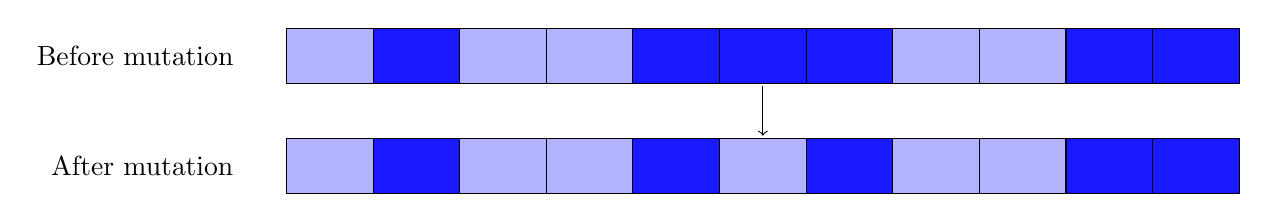
\begin{tikzpicture}[xscale=1.1,yscale=0.7]
\definecolor{b1}{rgb}{0.1,0.1,1}
\definecolor{b2}{rgb}{0.7,0.7,1}

\node[left] (bef) at (0,1) {Before mutation};
\node[left] (aft) at (0,-1) {After mutation};

\draw[fill=b2] (0.5,0.5) rectangle (1.5,1.5);
\draw[fill=b1] (1.5,0.5) rectangle (2.5,1.5);
\draw[fill=b2] (2.5,0.5) rectangle (3.5,1.5);
\draw[fill=b2] (3.5,0.5) rectangle (4.5,1.5);
\draw[fill=b1] (4.5,0.5) rectangle (5.5,1.5);
\draw[fill=b1] (5.5,0.5) rectangle (6.5,1.5);
\draw[fill=b1] (6.5,0.5) rectangle (7.5,1.5);
\draw[fill=b2] (7.5,0.5) rectangle (8.5,1.5);
\draw[fill=b2] (8.5,0.5) rectangle (9.5,1.5);
\draw[fill=b1] (9.5,0.5) rectangle (10.5,1.5);
\draw[fill=b1] (10.5,0.5) rectangle (11.5,1.5);

\draw[fill=b2] (0.5,-0.5) rectangle (1.5,-1.5);
\draw[fill=b1] (1.5,-0.5) rectangle (2.5,-1.5);
\draw[fill=b2] (2.5,-0.5) rectangle (3.5,-1.5);
\draw[fill=b2] (3.5,-0.5) rectangle (4.5,-1.5);
\draw[fill=b1] (4.5,-0.5) rectangle (5.5,-1.5);
\draw[fill=b2] (5.5,-0.5) rectangle (6.5,-1.5);
\draw[fill=b1] (6.5,-0.5) rectangle (7.5,-1.5);
\draw[fill=b2] (7.5,-0.5) rectangle (8.5,-1.5);
\draw[fill=b2] (8.5,-0.5) rectangle (9.5,-1.5);
\draw[fill=b1] (9.5,-0.5) rectangle (10.5,-1.5);
\draw[fill=b1] (10.5,-0.5) rectangle (11.5,-1.5);

\draw[->] (6,0.45) -- (6,-0.45);
\end{tikzpicture}
\caption{Schematic example of mutation in genetic algorithms}\label{Draw:8}
\end{figure}

\clearpage
% Draw:9
% Schematic example of mutation in genetic algorithms
\begin{figure}[!ht]
\centering
\footnotesize
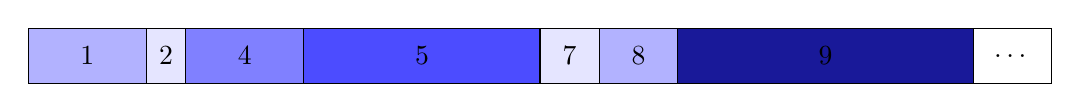
\begin{tikzpicture}[xscale=0.5,yscale=0.7]
\definecolor{b1}{rgb}{0.7,0.7,1}
\definecolor{b2}{rgb}{0.9,0.9,1}
\definecolor{b4}{rgb}{0.5,0.5,1}
\definecolor{b5}{rgb}{0.3,0.3,1}
\definecolor{b7}{rgb}{0.9,0.9,1}
\definecolor{b8}{rgb}{0.7,0.7,1}
\definecolor{b9}{rgb}{0.1,0.1,0.6}
\definecolor{b0}{rgb}{1,1,1}

\draw[fill=b1] (0,0) rectangle node {1} (3,1);
\draw[fill=b2] (3,0) rectangle node {2} (4,1);
\draw[fill=b4] (4,0) rectangle node {4} (7,1);
\draw[fill=b5] (7,0) rectangle node {5} (13,1);
\draw[fill=b7] (13,0) rectangle node {7} (14.5,1);
\draw[fill=b8] (14.5,0) rectangle node {8} (16.5,1);
\draw[fill=b9] (16.5,0) rectangle node {9} (24,1);
\draw[fill=b0] (24,0) rectangle node {\dots} (26,1);
\end{tikzpicture}
\caption{Schematic example of roulette wheel method}\label{Draw:9}
\end{figure}

\end{document}
